% ANUfinalexam.tex (Version 2.0)
% ===============================================================================
% Australian National University Final Exam LaTeX template.
% 2004; 2009, Timothy Kam, ANU School of Economics
% Licence type: Free as defined in the GNU General Public Licence: http://www.gnu.org/licenses/gpl.html

\documentclass[a4paper,12pt,fleqn]{article}
\setlength{\parindent}{0em}
\usepackage{amsmath}
\usepackage{fancyhdr}
\usepackage{siunitx}
\usepackage{enumitem}
\usepackage{amsmath}
\usepackage{graphicx}
\usepackage{tikz}
\usepackage{import}
\usepackage{comment}

% Unit definitions %%%%%%%%%%%%%%%%%%%%%%%%%%%%%%%%%%

\DeclareSIUnit\kilowatthour{kWh}
\DeclareSIUnit\kilowattpeak{kW_P}
\DeclareSIUnit\kVA{kVA}
\DeclareSIUnit\kVAR{kVAR}
\DeclareSIUnit\year{y}
\DeclareSIUnit\north{N}
\DeclareSIUnit\south{S}


% Insert your course information here %%%%%%%%%%%%%%%%%%%%%%%%%%%%%%%%%%

\newcommand{\institution}{CORNWALL COLLEGE}
\newcommand{\titlehd}{BSc Renewable Energy and Carbon Management}
\newcommand{\examtype}{Referral Assignment}
\newcommand{\examdate}{Academic Year 2014-2015}
\newcommand{\examcode}{CORC2086}
\newcommand{\examtitle}{Data Modelling and Processing}
\newcommand{\readtime}{15 Minutes}
\newcommand{\duedate}{Thursday $20^{\mathrm{th}}$ August 2015}
\newcommand{\materials}{Non-programmable Calculators; Formula Sheet}
\newcommand{\submission}{Please submit to the Assessment Moodle site by the due date}
\newcommand{\middlewords}{Assignment continues on next page}
\newcommand{\lastwords}{End of Assignment}

%%%%%%%%%%%%%%%%%%%%%%%%%%%%%%%%%%%%%%%%%%%%%%%%%%%%

%\setcounter{MaxMatrixCols}{10}
\newtheorem{theorem}{Theorem}
\newtheorem{acknowledgement}[theorem]{Acknowledgement}
\newtheorem{algorithm}[theorem]{Algorithm}
\newtheorem{axiom}[theorem]{Axiom}
\newtheorem{case}[theorem]{Case}
\newtheorem{claim}[theorem]{Claim}
\newtheorem{conclusion}[theorem]{Conclusion}
\newtheorem{condition}[theorem]{Condition}
\newtheorem{conjecture}[theorem]{Conjecture}
\newtheorem{corollary}[theorem]{Corollary}
\newtheorem{criterion}[theorem]{Criterion}
\newtheorem{definition}[theorem]{Definition}
\newtheorem{example}[theorem]{Example}
\newtheorem{exercise}[theorem]{Exercise}
\newtheorem{lemma}[theorem]{Lemma}
\newtheorem{notation}[theorem]{Notation}
\newtheorem{problem}[theorem]{Problem}
\newtheorem{proposition}[theorem]{Proposition}
\newtheorem{remark}[theorem]{Remark}
\newtheorem{solution}[theorem]{Solution}
\newtheorem{summary}[theorem]{Summary}
\newenvironment{proof}[1][Proof]{\noindent\textbf{#1.} }{\ \rule{0.5em}{0.5em}}

% ANU Exams Office mandated margins and footer style
\setlength{\topmargin}{0cm}
\setlength{\textheight}{9.25in}
\setlength{\oddsidemargin}{0.0in}
\setlength{\evensidemargin}{0.0in}
\setlength{\textwidth}{16cm}
\pagestyle{fancy}
\lhead{} 
\chead{} 
\rhead{} 
\lfoot{} 
\cfoot{\footnotesize{Page \thepage \ of \pageref{finalpage} -- \titlehd \ (\examcode)}} 
\rfoot{} 

% DEPRECATED: ANU Exams Office mandated margins and footer style
%\setlength{\topmargin}{0cm}
%\setlength{\textheight}{9.25in}
%\setlength{\oddsidemargin}{0.0in}
%\setlength{\evensidemargin}{0.0in}
%\setlength{\textwidth}{16cm}
%\pagestyle{fancy}
%\lhead{} %left of the header
%\chead{} %center of the header
%\rhead{} %right of the header
%\lfoot{} %left of the footer
%\cfoot{} %center of the footer
%\rfoot{Page \ \thepage \ of \ \pageref{finalpage} \\
%       \texttt{\examcode}} %Print the page number in the right footer

\renewcommand{\headrulewidth}{0pt} %Do not print a rule below the header
\renewcommand{\footrulewidth}{0pt}


\begin{document}

% Title page

\begin{center}
%\vspace{5cm}
\large\textbf{\institution}
\end{center}
\vspace{1cm}

\begin{center}
\textit{ \examtype -- \examdate}
\end{center}
\vspace{1cm}

\begin{center}
\large\textbf{\titlehd}
\end{center}

\begin{center}
\large\textbf{\examcode}
\end{center}
\begin{center}
\large\textbf{\examtitle}
\end{center}

\vspace{2 cm}

\begin{center}
\textit{Due date:  \duedate}
\end{center}

%\begin{center}
%\textit{Submission:  \submission}
%\end{center}

\vspace{2cm}

\textbf{Instructions}

\begin{quote}
\textit{Answer\textbf{\ all} parts of the question. Please organise your spreadsheet so that it is easy to read and follow.\\Please submit your finished  spreadsheet to the usual assessment page on the Moodle site for the course by 23:55 on the due date}
\end{quote}

\textbf{Assessment Criteria}

\begin{itemize}
\item Use of suitable look-up and other formulae in your spreadsheet
\item Elegance of your spreadsheet solutions
\item Flexibility of your spreadsheet solutions: how easily could they be adapted to another, similar problem?
\item Clarity of your graphical figures
\item Sensible estimates of annual energy production: how fully have you realised the control regime and complied with the technical and regulatory limitations?
\item Use of appropriate sources – for example for feed-in tariff and any other income that the scheme might generate. 
\end{itemize}

% End title page

\textbf{Data analysis for a  hydroelectric scheme}
\newline\newline
A hydroelectric scheme is proposed for a river in Cornwall with an effective head height of \SI{23.8}{\metre}. The Environment Agency has stipulated that the depleted stretch of the river should have a hands off flow rate of \SI{238}{\litre\per\second} in the winter and \SI{334}{\litre\per\second} in the summer.
\newline\newline
The turbines to be used are three KSB Etanorm R-200-260 motor/pump combinations that it is proposed to use as turbine/generators. The total power output of the scheme must not exceed \SI{100}{\kilo\watt} at any one time in order for it to attract the feed-in tariff.
\newline\newline
A control system is to be used that will allow each turbine to be turned on/off individually as flow conditions vary, and to limit the total shaft output power to \SI{100}{\kilo\watt}.
\newline\newline
Figure \ref{fig:ksb} shows a picture of one of these pumps installed as a turbine, with generator attached.

\begin{figure}[h]
\centering
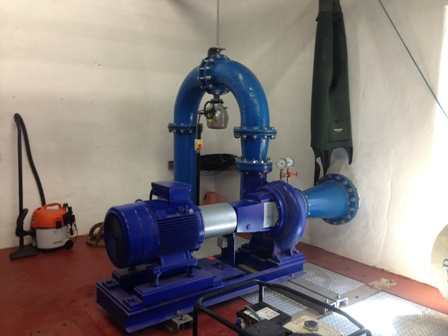
\includegraphics[width=0.5\textwidth]{./figures/ksb-pump}
\caption{KSB pump, used as a turbine, with generator attached}
\label{fig:ksb}
\end{figure}

You are provided with the following data:
\begin{itemize}
\item Flow rate data for the river with daily resolution for the period 1969 to 2010
\item Flow rate data for the river for the year 2012 with 15 minute resolution.
\end{itemize}

Both these data sets were measured at a gauging station at a site further upstream from the proposed scheme. At the site of the scheme, the catchment area is 1.46 times that at the gauging station. 
\newline\newline
Power curve data for a KSB Etanorm R-200-260 motor/pump combination that it is proposed to use as a turbine/ generator. The control system is set up such that each turbine can only operate in the range \SI{160}{\litre\per\second} to \SI{220}{\litre\per\second}.

\newpage
\textbf{Tasks}
\newline\newline

\begin{enumerate}[label=\alph*)]
\item Find the daily average flow rates of the river in 2012. [20\%] 
\item Produce an annual hydrograph for the river for 2012. [20\%]
\item Produce a flow duration curve for the river for 2012. [20\%]
\item Using Solver in Excel or otherwise, fit a Weibull probability distribution curve to the measured flow probability distribution and establish the best fit values for this river of the shape parameter k and the scale parameter A. Calculate $R^2$ for the fit to establish whether the fit is good or not. [20\%]
\item Using the fit parameters found in (4), estimate the annual energy production and income from the scheme in 2015, given a control regime whereby at most one turbine is running at part load at any one time. Note that the total output power of the turbines must not exceed \SI{100}{\kilo\watt} at any time. [20\%]
\end{enumerate}

You must submit a spreadsheet for this task to the Moodle assignment submission site, by midnight on the deadline. The spreadsheet must contain all calculations and figures. Any explanatory text should be included as text boxes within the spreadsheet. 

\label{finalpage}

\end{document}

